% -*- latex -*-
%%%%%%%%%%%%%%%%%%%%%%%%%%%%%%%%%%%%%%%%%%%%%%%%%%%%%%%%%%%%%%%%
%%%%%%%%%%%%%%%%%%%%%%%%%%%%%%%%%%%%%%%%%%%%%%%%%%%%%%%%%%%%%%%%
%%%%
%%%% This text file is part of the source of slides for
%%%% `The Art of HPC, vol 1: The Science of Computing'
%%%% by Victor Eijkhout, copyright 2012-2024
%%%%
%%%%%%%%%%%%%%%%%%%%%%%%%%%%%%%%%%%%%%%%%%%%%%%%%%%%%%%%%%%%%%%%
%%%%%%%%%%%%%%%%%%%%%%%%%%%%%%%%%%%%%%%%%%%%%%%%%%%%%%%%%%%%%%%%

\Level 1 {Collectives as building blocks; complexity}

\begin{frame}[containsverbatim]\frametitle{Collectives}
  Gathering and spreading information:
  \begin{itemize}
  \item Every process has data, you want to bring it together;
  \item One process has data, you want to spread it around.
  \end{itemize}
  Root process: the one doing the collecting or disseminating.

  Basic cases:
  \begin{itemize}
  \item Collect data: gather.
  \item Collect data and compute some overall value (sum, max): reduction.
  \item Send the same data to everyone: broadcast.
  \item Send individual data to each process: scatter.
  \end{itemize}
\end{frame}

\frame{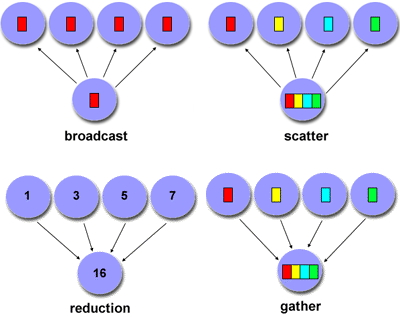
\includegraphics[scale=.5]{collective_comm}}

\begin{frame}{Collective scenarios}
  How would you realize the following scenarios with collectives?
  \begin{itemize}
  \item Let each process compute a random number. You want to print the
    maximum of these numbers to your screen.
  \item Each process computes a random number again. Now you want to
    scale these numbers by their maximum. 
  \item Let each process compute a random number. You want to print on what processor the
    maximum value is computed. 
  \end{itemize}
\end{frame}

\begin{frame}{Simple model of parallel computation}
\begin{itemize}
\item $\alpha$: message latency
\item $\beta$: time per word (inverse of bandwidth)
\item $\gamma$: time per floating point operation
\end{itemize}
Send $n$ items and do $m$ operations:
\[ \mathit{cost}=\alpha+\beta\cdot n +\gamma\cdot m \]
Pure sends: no $\gamma$ term,\\
pure computation: no $\alpha,\beta$ terms,\\
sometimes mixed: reduction
\end{frame}

\begin{frame}{Model for collectives}
\begin{itemize}
\item One simultaneous send and receive:
\item doubling of active processors
\item collectives have a $\alpha\log_2 p$ cost component
\end{itemize}

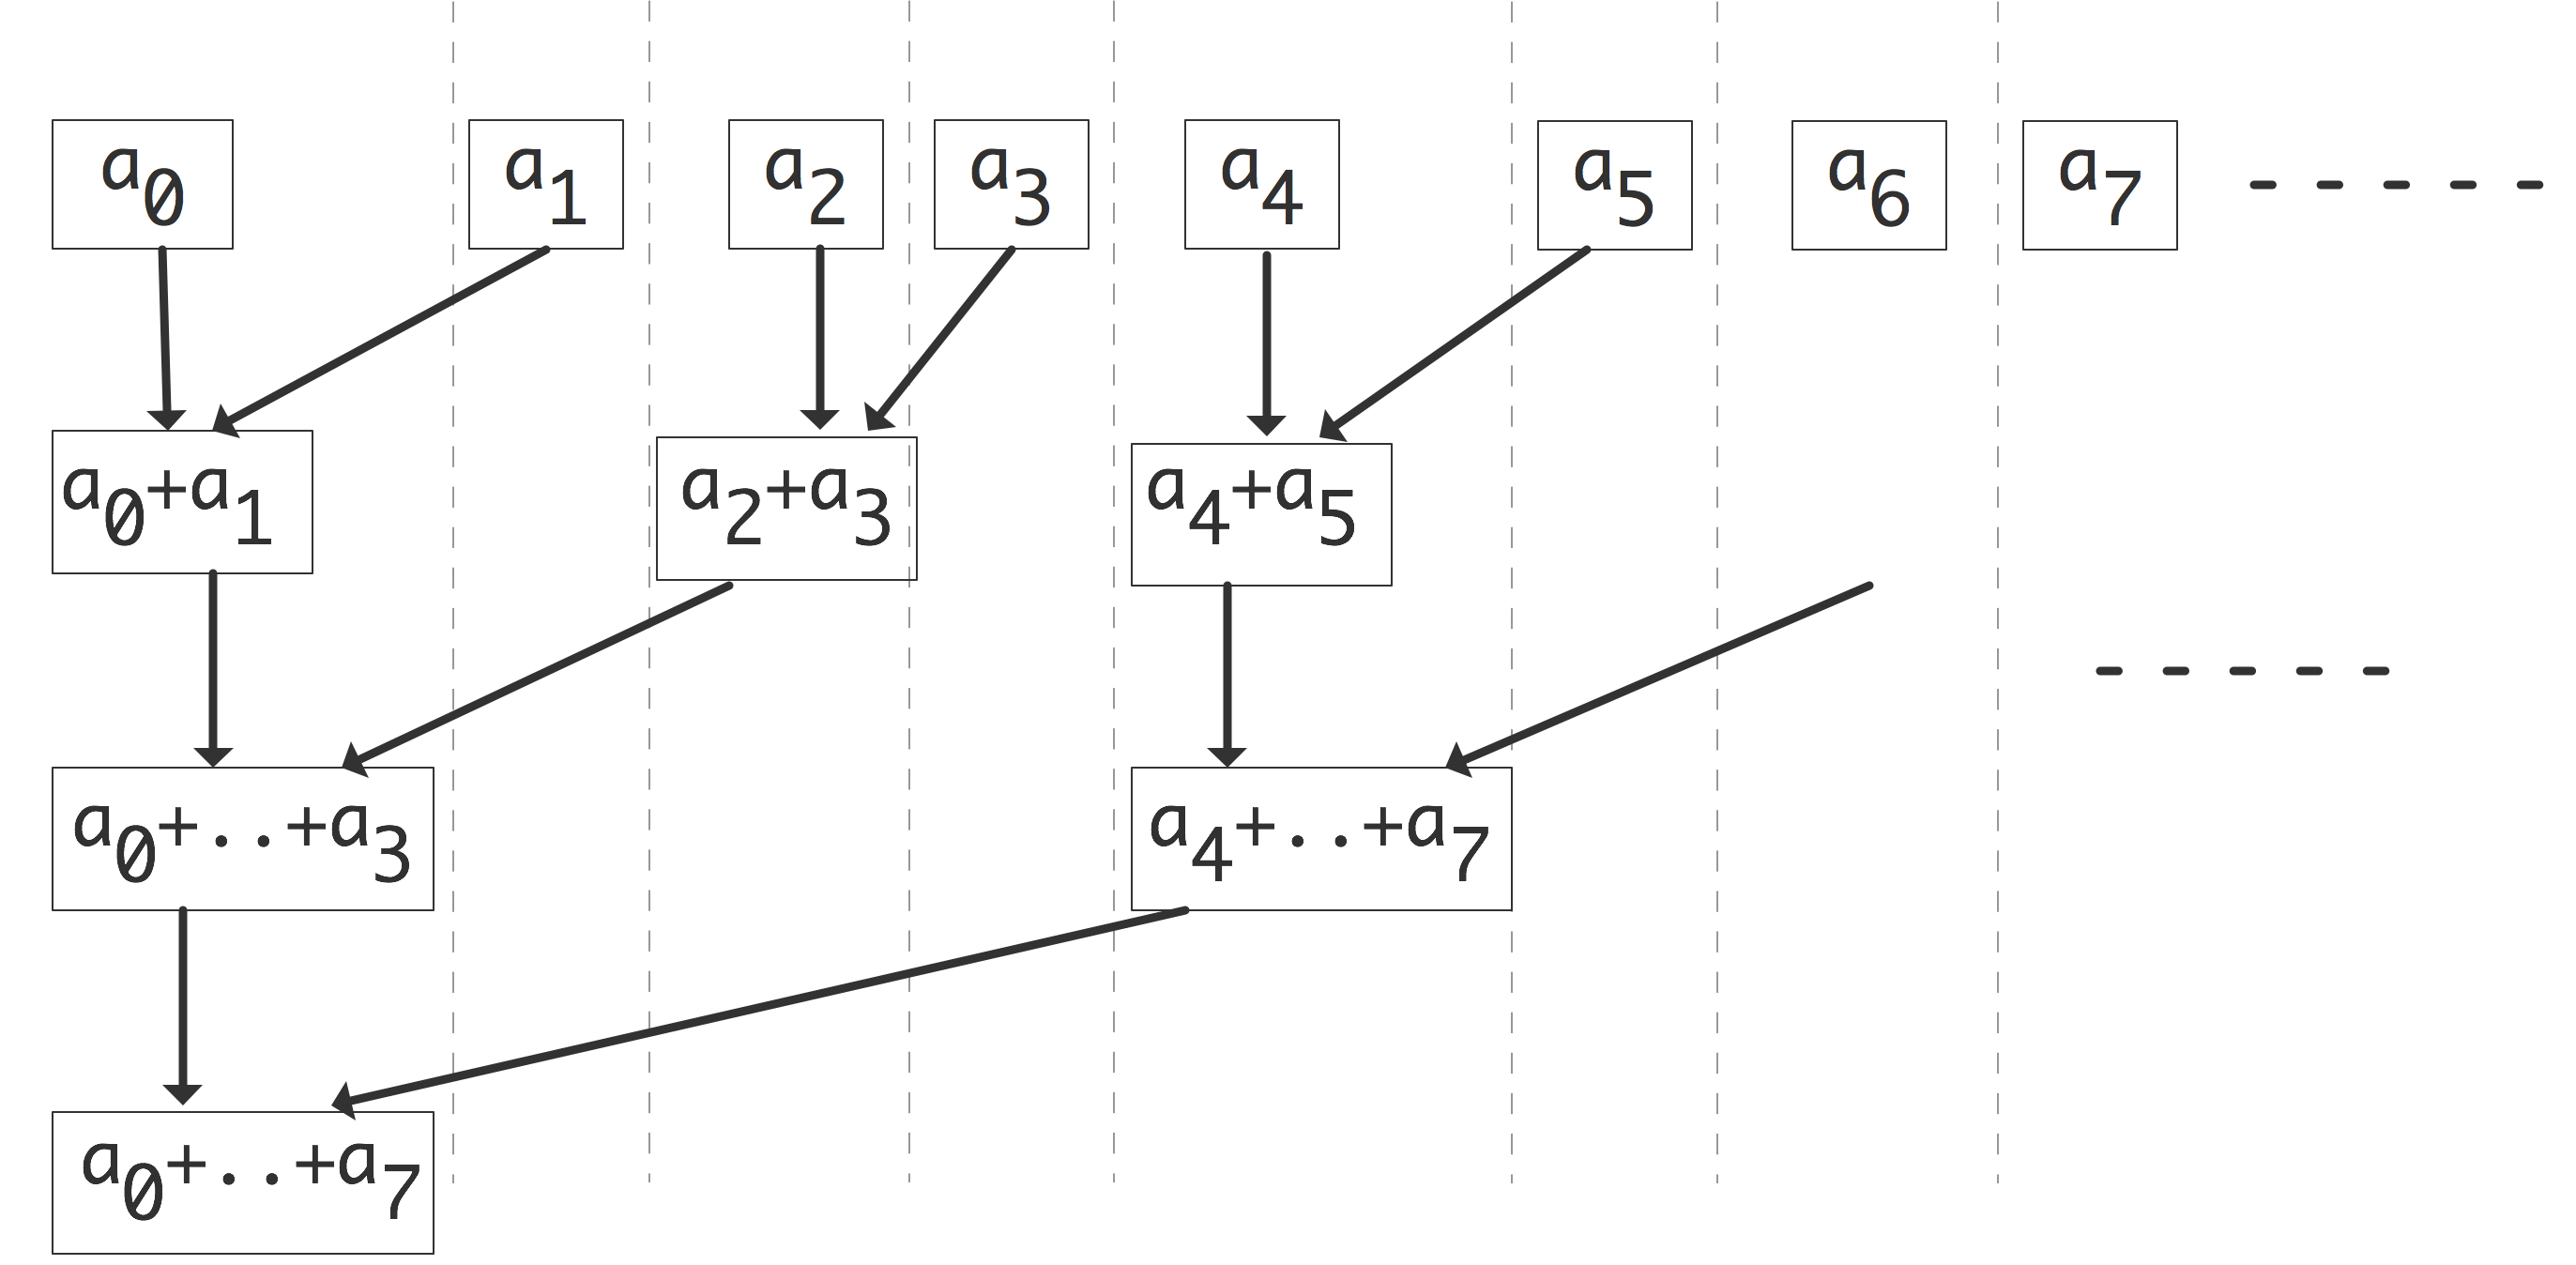
\includegraphics[scale=.1]{parallel-sum-graph}
\end{frame}

\begin{frame}{Broadcast}
\[
\begin{array}{|c|ccc|}
\hline
  &t=0&t=1&t=2\\ \hline
p_0&x_0\downarrow,x_1\downarrow,x_2\downarrow,x_3\downarrow
   &x_0\downarrow,x_1\downarrow,x_2\downarrow,x_3\downarrow
   &x_0,x_1,x_2,x_3\\
p_1&&x_0\downarrow,x_1\downarrow,x_2\downarrow,x_3\downarrow
   &x_0,x_1,x_2,x_3\\
p_2&&&x_0,x_1,x_2,x_3\\
p_3&&&x_0,x_1,x_2,x_3\\
\hline
\end{array}
\]
On $t=0$, $p_0$ sends to $p_1$; on $t=1$ $p_0,p_1$ send to $p_2,p_3$.

Optimal complexity:
\[ \lceil\log_2 p\rceil \alpha+n\beta. \]
Actual complexity:
\[ \lceil\log_2 p\rceil (\alpha+n\beta). \]
Good enough for short vectors.
\end{frame}

\begin{frame}{Long vector broadcast}
  Start with a scatter:
\[
\begin{array}{|c|cccc|}
\hline
  &t=0&t=1&t=2&t=3\\ \hline
  p_0&x_0\downarrow,x_1,x_2,x_3 % t=0
  &x_0,x_1\downarrow,x_2,x_3 % t=1
   &x_0,x_1,x_2\downarrow,x_3 % t=2
  &x_0,x_1,x_2,x_3\downarrow % t=3
  \\
  p_1& % t=0
  &x_1&&\\
  p_2&& % t=0,1
  &x_2&\\
  p_3&&& % t=0,1,2
  &x_3\\
\hline
\end{array}
\]
takes $p-1$ messages of size $N/p$, for a total time of
\[ T_{\scriptsize\mathrm{scatter}}(N,P) = (p-1)\alpha +
(p-1)\cdot\frac{N}{p}\cdot \beta.
\]
\end{frame}

\begin{frame}{Bucket brigade}
  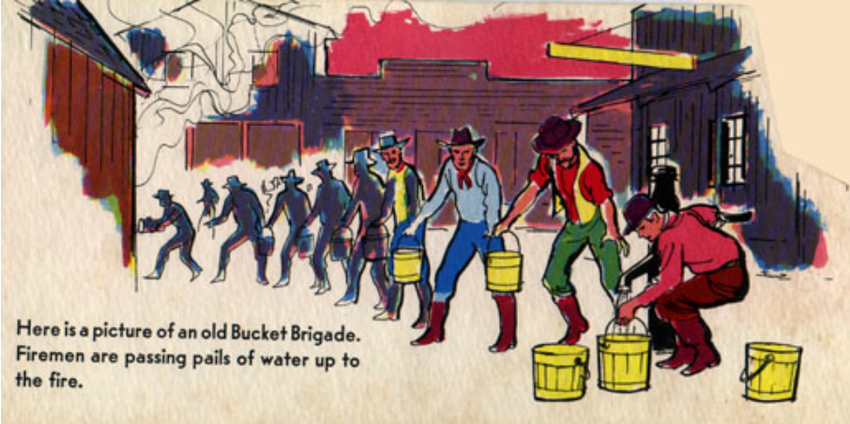
\includegraphics[scale=.3]{bucketbrigade}
\end{frame}

\begin{frame}{Long vector broadcast}
  After the scatter do a bucket-allgather:
\[
\begin{array}{|c|lll|}
\hline
  &t=0&t=1&et cetera\\ \hline
p_0&x_0\downarrow\hphantom{,x_1\downarrow,x_2\downarrow,x_3\downarrow}
   &x_0\hphantom{\downarrow,x_1\downarrow,x_2\downarrow,}x_3\downarrow
   &x_0,\hphantom{x_1,}x_2,x_3\\
p_1&\hphantom{x_0\downarrow,}x_1\downarrow\hphantom{,x_2\downarrow,x_3\downarrow}
   &x_0\downarrow,x_1\hphantom{\downarrow,x_2\downarrow,x_3\downarrow}
   &x_0,x_1,\hphantom{x_2,}x_3\\
p_2&\hphantom{x_0\downarrow,x_1\downarrow,}x_2\downarrow\hphantom{,x_3\downarrow}
   &\hphantom{x_0\downarrow,}x_1\downarrow,x_2\hphantom{\downarrow,x_3\downarrow}
   &x_0,x_1,x_2\hphantom{,x_3}\\
p_3&\hphantom{x_0\downarrow,x_1\downarrow,x_2\downarrow,}x_3\downarrow
   &\hphantom{x_0\downarrow,x_1\downarrow,}x_2\downarrow,x_3\hphantom{\downarrow}
   &\hphantom{x_0,}x_1,x_2,x_3\\
\hline
\end{array}
\]
Each partial message gets sent $p-1$ times, so this stage also has a
complexity of 
\[ T_{\scriptsize\mathrm{bucket}}(N,P) = (p-1)\alpha +
(p-1)\cdot\frac{N}{p}\cdot \beta.
\]
  Better if $N$ large.
\end{frame}

\begin{frame}{Reduce}
\small
Optimal complexity:
    \[ \lceil\log_2 p\rceil \alpha+n\beta +\frac{p-1}p \gamma n. \]
Spanning tree algorithm:
{\small
\[ \kern-.2in
\begin{array}{|c|ccc|}
\hline
  &t=1&t=2&t=3\\ \hline
p_0&x_0^{(0)},x_1^{(0)},x_2^{(0)},x_3^{(0)}
   &x_0^{(0:1)},x_1^{(0:1)},x_2^{(0:1)},x_3^{(0:1)}
   &x_0^{(0:3)},x_1^{(0:3)},x_2^{(0:3)},x_3^{(0:3)}\\
p_1&x_0^{(1)}\uparrow,x_1^{(1)}\uparrow,x_2^{(1)}\uparrow,x_3^{(1)}\uparrow
   &&\\
p_2&x_0^{(2)},x_1^{(2)},x_2^{(2)},x_3^{(2)}
   &x_0^{(2:3)}\uparrow,x_1^{(2:3)}\uparrow,x_2^{(2:3)}\uparrow,x_3^{(2:3)}\uparrow
   &\\
p_3&x_0^{(3)}\uparrow,x_1^{(3)}\uparrow,x_2^{(3)}\uparrow,x_3^{(3)}\uparrow
   &&\\
\hline
\end{array}
\]
}
Running time
    \[ \lceil\log_2 p\rceil (\alpha+n\beta +\frac{p-1}p \gamma n). \]
Good enough for short vectors.
\end{frame}

\begin{frame}{Allreduce}
  Allreduce~$\equiv$ Reduce$+$Broadcast

{\tiny
\input allreduce
}

Same running time as regular reduce!
\end{frame}

\begin{frame}{Allgather}
Gather $n$ elements: each processor owns $n/p$;\\
optimal running time
\[ \lceil \log_2 p\rceil\alpha +\frac{p-1}pn\beta. \]
\[
\begin{array}{|c|ccc|}
\hline
  &t=1&t=2&t=3\\ \hline
p_0&x_0\downarrow&x_0x_1\downarrow&x_0x_1x_2x_3\\
p_1&x_1\uparrow&x_0x_1\downarrow&x_0x_1x_2x_3\\
p_2&x_2\downarrow&x_2x_3\uparrow&x_0x_1x_2x_3\\
p_3&x_3\uparrow&x_2x_3\uparrow&x_0x_1x_2x_3\\
\hline
\end{array}
\]
Same time as gather, half of gather-and-broadcast.
\end{frame}

\begin{frame}{Reduce-scatter}
\small 
\[ \kern-.25in
\begin{array}{|c|ccc|}
\hline
  &t=1&t=2&t=3\\ \hline
p_0&x_0^{(0)},x_1^{(0)},x_2^{(0)}\downarrow,x_3^{(0)}\downarrow
   &x_0^{(0:2:2)},x_1^{(0:2:2)}\downarrow
    \hphantom{x_0^{(0:2:2)},x_1^{(0:2:2)}\downarrow}
   &x_0^{(0:3)}
    \hphantom{x_3^{(0:3)}x_3^{(0:3)}x_3^{(0:3)}}\\
p_1&x_0^{(1)},x_1^{(1)},x_2^{(1)}\downarrow,x_3^{(1)}\downarrow
   &x_0^{(1:3:2)}\uparrow,x_1^{(1:3:2)}
    \hphantom{x_0^{(0:2:2)},x_1^{(0:2:2)}\downarrow}
   &\hphantom{x_3^{(0:3)}} x_1^{(0:3)}
    \hphantom{x_3^{(0:3)}x_3^{(0:3)}} \\
p_2&x_0^{(2)}\uparrow,x_1^{(2)}\uparrow,x_2^{(2)},x_3^{(2)}
   &\hphantom{x_0^{(0:2:2)},x_1^{(0:2:2)}\downarrow}
    x_2^{(0:2:2)},x_3^{(0:2:2)}\downarrow
   &\hphantom{x_3^{(0:3)}x_3^{(0:3)}} x_2^{(0:3)}
    \hphantom{x_3^{(0:3)}}\\
p_3&x_0^{(3)}\uparrow,x_1^{(3)}\uparrow,x_2^{(3)},x_3^{(3)}
   &\hphantom{x_0^{(0:2:2)},x_1^{(0:2:2)}\downarrow}
    x_0^{(1:3:2)}\uparrow,x_1^{(1:3:2)}
   &\hphantom{x_3^{(0:3)}x_3^{(0:3)}x_3^{(0:3)}}
    x_3^{(0:3)}\\
\hline
\end{array}
\]
\[ \lceil \log_2 p\rceil\alpha +\frac{p-1}pn(\beta+\gamma). \]
\end{frame}

